\documentclass[11pt,parskip=full]{scrartcl}%article}
%\setlength{\parskip}{1em}

%%%%%%%%%%%%%%%%%%%%%%
%% PACKAGE INCLUDES %%
%%%%%%%%%%%%%%%%%%%%%%

\usepackage{array}           % For defining \newcolumntype.
\usepackage{amsmath}
\usepackage{amssymb}
\usepackage{amsthm}          % Provides 'proof' environment.
\usepackage[english]{babel}  % For defining 'theorem/corollary/lemma' environments.
\usepackage{bm}              % Provides bold \pi
\usepackage{booktabs}
\usepackage{hyperref}
\usepackage{gensymb}         % Enables \degree command for °C.
\usepackage{todonotes}
\usepackage{subfig}
\usepackage{enumitem}


%%%%%%%%%%%%%%%%%
%% STYLE SETUP %%
%%%%%%%%%%%%%%%%%

% Define some custom colors.
\definecolor{mylinkcolor}{RGB}{000, 114, 166}
\definecolor{mycitecolor}{RGB}{255, 154, 071}
\definecolor{myurlcolor}{RGB}{000, 114, 166}

% Set itemize format.
\setitemize{noitemsep,topsep=-5pt,parsep=5pt,partopsep=0pt}

% Define column types that allow fixed width params.
\newcolumntype{L}[1]{>{\raggedright\let\newline\\\arraybackslash\hspace{0pt}}m{#1}}
\newcolumntype{C}[1]{>{\centering\let\newline\\\arraybackslash\hspace{0pt}}m{#1}}
\newcolumntype{R}[1]{>{\raggedleft\let\newline\\\arraybackslash\hspace{0pt}}m{#1}}

% Color setup for hyperlinks/references/citations/urls.
\hypersetup{
    colorlinks,
    linkcolor={mylinkcolor},
    citecolor={mycitecolor},
    urlcolor={myurlcolor}
}

% Specify hyphenation of words on line break.
\hyphenation{Figure Table Chapter Section}



%%%%%%%%%%%%
%% MACROS %%
%%%%%%%%%%%%

% Set default font family to sans-serif.
\renewcommand*{\familydefault}{\sfdefault}

\newcommand*{\ie}{i.e., }
\newcommand*{\eg}{e.g., }
\newcommand*{\wrt}{with respect to }

\newcommand*{\tokens}{\mathcal{T}}          % Set of tokens.
\newcommand*{\orders}{\mathcal{O}}          % Set of orders.
\newcommand*{\itokens}{\mathcal{I}^t}       % Set of token indices.
\newcommand*{\itokenpairs}{\mathcal{I}^p}   % Set of token index pairs.
\newcommand*{\iutokenpairs}{\tilde{\mathcal{I}}^p}   % Set of token index pairs.
\newcommand*{\iorders}{\mathcal{I}^o}       % Set of order indices.
\newcommand*{\ibuyorders}{\mathcal{I}^b}    % Set of buy order indices.
\newcommand*{\isellorders}{\mathcal{I}^s}   % Set of sell order indices.

% Macros for references etc.
\newcommand*{\figref}[1]{\hyperref[{#1}]{Figure~\ref*{#1}}}
\newcommand*{\tabref}[1]{\hyperref[{#1}]{Table~\ref*{#1}}}
\newcommand*{\secref}[1]{\hyperref[{#1}]{Section~\ref*{#1}}}
\newcommand*{\subsecref}[1]{\hyperref[{#1}]{Section~\ref*{#1}}}
\newcommand*{\thmref}[1]{\hyperref[{#1}]{Theorem~\ref*{#1}}}
\newcommand*{\crlref}[1]{\hyperref[{#1}]{Corollary~\ref*{#1}}}
\newcommand*{\lemref}[1]{\hyperref[{#1}]{Lemma~\ref*{#1}}}

% Macros for theorems|corollaries|lemmas|observations.
\newtheorem{theorem}{Theorem}[section]
\newtheorem{corollary}{Corollary}[theorem]
\newtheorem{lemma}[theorem]{Lemma}
\newtheorem{observation}[theorem]{Observation}

%%%%%%%%%%%%%%
%% DOCUMENT %%
%%%%%%%%%%%%%%

\title{
  Multi-token Batch Auctions with Uniform Clearing Prices\\
  - \\
  \Large Features and Models}
\author{Tom Walther \\ tom@gnosis.pm}

\date{\today}



\begin{document}

\maketitle


\begin{abstract}
  This document describes the problem of multi-token batch auctions with uniform clearing prices as
  a price-finding mechanism proposed for a decentralized token trading platform.
  Moreover, it contains solution approaches based on combinatorial optimization formulations, as
  well as some computational results.
%\footnote{... footnote ...}.
\end{abstract}

%\todo[inline,caption={}]{
%  \begin{itemize}
%    \item computational results for MIP\{2|3\}
%  \end{itemize}
%}


\tableofcontents

\newpage
\section{Introduction}
\label{sec:introduction}

In continuous-time token exchange mechanisms, orders are typically collected in order books of two
tokens that are traded against each other.
A trade happens whenever a buy order of one token is matched by a sell order of the other, \ie if
there exists an exchange rate that satisfies the limit prices stated in the respective orders.
In a setting of multiple tradeable tokens, one separate order book is required for every token pair
combination.
This may significantly limit liquidity for less frequently traded token pairs and lead to large
bid-ask spreads and low trading volumes.

In our approach, we want to collect orders for a set of multiple tokens in a single joint order
book and compute exchange prices for all token pairs simultaneously at the end of discrete time
intervals (\emph{multi-token batch auction}).
Trades between the same token pairs are then all executed at the same exchange rate (\emph{uniform
clearing price}).
Moreover, this mechanism enables so-called \emph{ring trades}, where orders are matched along
cycles of tokens.
In order to exclude arbitrage opportunities, we require prices to be consistent along such cycles,
\ie we want the constraint
\begin{align}
  p_{j|k} \cdot p_{k|l} = p_{j|l}
  \label{eq:arbitrage_freeness}
\end{align}
to be satisfied for the prices of all tokens j,k,l.

The concept of frequent batch auctions aiming at reducing arbitrage and improving liquidity has
been investigated extensively in \cite{budish:HFT}.
Moreover, the advantages of uniform-price clearing have been discussed in 
\cite{engelbrecht:multi_unit_auctions}.
In this document, we want to describe the problem of determining uniform clearing prices for all
pairs of tokens involved in a multi-token batch auction process, and present a mixed-integer
programming (MIP) solution approach.


\clearpage
\section{Problem statement}
\label{sec:problem}

\subsection{Data}
\label{subsec:data}

Let $ \tokens := \{ \tau_1 \ldots \tau_n \} $ denote the set of the $ n $ tokens that we want to
consider.
Additionally, we introduce an artificial token~$ \tau_0 $ that shall be referred to as 
\emph{reference token}, which will become important in our modelling approaches later on in 
\secref{sec:models}.
For convenience of notation, we use $ \mathcal{I}^t := \{ 1 \ldots n \} $ to denote the indices
of our token set.

Pairwise exchange rates between two tokens $ \tau_j $ and $ \tau_k $ will be denoted by
$ p_{j|k} $, meaning the price of one unit of $ \tau_j $ measured in units of $ \tau_k $.
As an example, if $ p_{j|k} = 10 $, one would need to pay an amount of $ 10 $ units of $ \tau_k $
in order to purchase one unit of $ \tau_j $.

Let there be a set $ \orders = \{ \omega_1 \ldots \omega_N \} $ of $ N $ limit orders in the batch
to be processed and let $ \ibuyorders, \isellorders \subseteq \{ 1 \ldots N \} =: \iorders $ denote
the sets of indices of buy and sell orders, respectively.
Every order must be of exactly one of the two types, so $ \ibuyorders \cap \isellorders =
\emptyset $ and $ \ibuyorders \cup \isellorders = \{ 1 \ldots N \} $.

Moreover, every buy order consists of a tuple $ (j,k,\overline{x},\pi) $ that is to be read as
\vspace{-.6cm}
\begin{center}
  \emph{
    "Buy (at most) $ \overline{x} $ units of token $ \tau_j $ for token $ \tau_k $
    if the rate $ p_{j|k} $ is at most $ \pi $".
  }
\end{center}
\vspace{-.4cm}
Analogously, every sell order is represented by a tuple $ (j,k,\overline{y},\pi) $ with the meaning
\vspace{-.6cm}
\begin{center}
  \emph{
    "Sell (at most) $ \overline{y} $ units of token $ \tau_j $ for token $ \tau_k $
    if the rate $ p_{j|k} $ is at least $ \pi $".
  }
\end{center}
\vspace{-.3cm}

The semantics of the two order types are somewhat similar in that there is one token to be
exchanged against another, if a certain limit price is guaranteed.
Such orders are hence referred to as \emph{limit orders}.
The difference between buy and sell orders is the following:
\begin{itemize}
  \item In a buy order, a fixed (maximum) buy volume $ \overline{x} $ is set, so the buyer
  indicates a preference to buy $ \overline{x} $ units of token $ \tau_j $.
  The amount of units of token $ \tau_k $ to be sold is flexible, as long as the limit price is
  respected (the smaller, the better).
  \item In a sell order, a fixed (maximum) sell volume $ \overline{y} $ is set, so the seller
  indicates a preference to sell $ \overline{y} $ units of token $ \tau_j $.
  The amount of units of token $ \tau_k $ to be bought is flexible, as long as the limit price
  is respected (the higher, the better).
\end{itemize}
\vspace{.3cm}

Nevertheless, the question remains whether it makes sense to keep the distinction between buy and
sell orders.
Consider a buy order $ (j,k,\overline{x},\pi) $, which reveals that the buyer would be ready to
sell at most $ \pi \cdot \overline{x} $ tokens $ \tau_k $ in exchange for tokens $ \tau_j $.
Then, from an economically rational point of view, the buyer should not object to receiving more
than $ \overline{x} $ tokens $ \tau_j $ for a maximum of $ \pi \cdot \overline{x} $ tokens
$ \tau_k $, \ie if the exchange rate $ p_{j|k} $ is lower than $ \pi $.
Hence, the buy order could be translated into an equivalent sell order
$ (k,j,\pi \cdot \overline{x},\pi) $.
In this paper, however, we will continue to treat the different order types separately.


\subsection{Objectives}
\label{subsec:objectives}

Having collected a batch of buy and sell orders for our set of tokens, we ultimately want to
compute exchange rates for all token pairs.
Therefore, the following optimization criteria could be used:
\begin{itemize}
  \item maximize the amount of trade that is enabled (\wrt some reference token)
  \item maximize \emph{trader welfare}, \eg defined as difference of paid price vs. limit price
\end{itemize}


\subsection{Constraints}
\label{subsec:constraints}

The solution that we are aiming at needs to satisfy several requirements that can be stated on a
high level as follows:
\begin{itemize}
  \item \emph{(buy limit price)}:\\
  for all buy orders
  $ \omega_i = (j_i,k_i,\overline{x}_i,\pi_i)  \in \orders, \> i \in \ibuyorders $:
  the order can only be executed (fully or fractionally) if the exchange rate does not exceed the
  limit price, \ie $ p_{j_i|k_i} \le \pi $.
  \item \emph{(sell limit price)}:\\
  for all sell orders
  $ \omega_i = (j_i,k_i,\overline{y}_i,\pi_i)  \in \orders, \> i \in \ibuyorders $:
  the order can only be executed (fully or fractionally) if the exchange rate is not lower than the
  limit price, \ie $ p_{j_i|k_i} \ge \pi $.
  \item \emph{(token balance)}:\\
  for every token $ \tau_j \in \tokens $: the amount of tokens $ \tau_j $ that were bought must
  equal the amount of tokens $ \tau_j $ that were sold.
  \item \emph{(price coherence)}:\\
  for all token pairs $ (\tau_j,\tau_k) $: $ p_{j|k} \cdot p_{k|j} = 1 $.
  \item \emph{(arbitrage freeness)}:\\
  for all token triples $ (\tau_j,\tau_k,\tau_l) $: $ p_{j|k} \cdot p_{k|l} = p_{j|l} $.
\end{itemize}

\vspace{.6cm}
\begin{lemma}
  (arbitrage freeness) $ \Rightarrow $ (price coherence).
\end{lemma}
\vspace{-.8cm}
\begin{proof}
  Consider three tokens $ \{\tau_j,\tau_k,\tau_l\} \subset \tokens $.
  We apply the arbitrage-freeness condition twice:
  \begin{itemize}
    \item[(i)] $ p_{j|k} \cdot p_{k|l} = p_{j|l} $
    \item[(ii)] $ p_{j|l} \cdot p_{l|k} = p_{j|k} $
  \end{itemize}
  Inserting (i) into (ii) and assuming prices to be strictly positive yields
  \begin{align*}
    p_{j|k} \cdot p_{k|l} \cdot p_{l|k} = p_{j|k}
    \qquad \Leftrightarrow \qquad
    p_{k|l} \cdot p_{l|k} = 1
  \end{align*}
\end{proof}
\vspace{-.4cm}

Notice that the above constraints also imply $ p_{j|j} = 1 $ for every
token~$ \tau_j \in \tokens $.

\subsection{Properties}
\label{subsec:properties}

Here is a list of research questions that we would like to answer.

\begin{itemize}
  \item In an optimal solution, is it guaranteed that orders can always be fully executed if their
  limit prices are strictly higher (buy order) or lower (sell order) than the exchange rate between
  the respective token pair?
  If true, we would only need to resort to partially executing orders if the execution price is
  equal to the limit price.
  \item What is the impact of optimizing the trading volume vs. the traders' welfare?
\end{itemize}


\subsection{Example}
\label{subsec:example}

A typical instance of our batch auction problem could look like shown in 
\figref{fig:order-token-graph}.
It is assumed that some token pairs will encounter high trading demand whereas other will only
rarely be traded on.

\begin{figure}[h!]
  \centering
  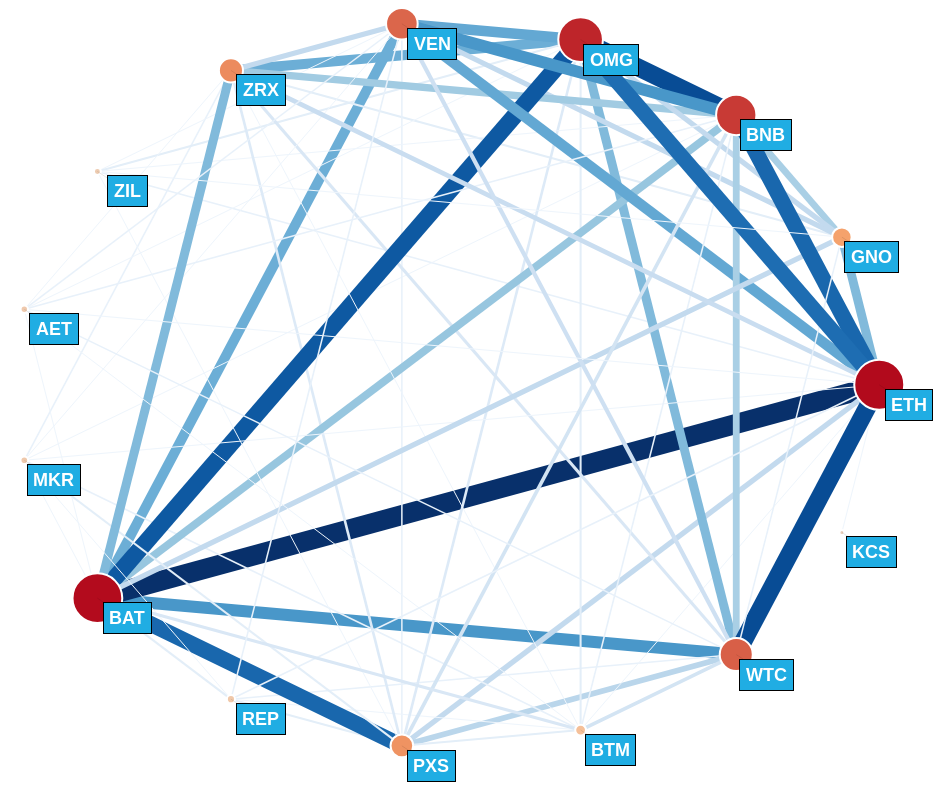
\includegraphics[width=.82\textwidth]{figures/token_order_graph.png}
  \caption{Token-order-graph representing a multi-token batch auction instance. Nodes correspond
  to tokens (with their size indicating the trading demand), the thickness of an edge represents 
  the number of orders placed on the respective token pair.}
  \label{fig:order-token-graph}
\end{figure}

\clearpage
\section{Models and Formulations}
\label{sec:models}

In this section, we want to present and discuss several solution approaches for our batch auction
problem, mainly in terms of mathematical optimization formulations.
We will begin with a nonlinear programming formulation (NLP) and proceed with mixed-integer linear
(MIP) and network flow formulations thereafter.

With the exchange rates between pairs of tokens being variables, modelling arbitrage-freeness
constraints of type \eqref{eq:arbitrage_freeness} intuitively leads to many multiplications being
required.
This may result in unnecessary limitations to the problem size that is tractable as well as
numerical instability.
However, we can do better by not considering all pairwise token rates explicitely but representing
all token prices only with respect to a single reference token $ \tau_0 $.
Let $ p_j := p_{j|0} $ denote the price of token $ \tau_j $ expressed in units of token $ \tau_0 $ 
(hence, $ p_0 = 1 $).
Applying the arbitrage-freeness and price-coherence conditions directly, we can express the
exchange rate between two tokens $ \tau_j $ and $ \tau_k $ as
\begin{align}
  p_{j|k} = p_{j|0} \cdot p_{0|k} = \frac{p_{j|0}}{p_{k|0}} = \frac{p_j}{p_k}.
\end{align}

We now have some freedom to decide what exactly the artificial reference token should represent.
For example, we could select one particular $ \tau_j \in \tokens $ to be the reference, \ie
\begin{subequations}
\begin{align}
  p_0 &= p_j.
  \label{eq:refToken_1}
\end{align}
Then, all trading volume would be computed \wrt $ \tau_j $ (which we will explain later in the
model formulation sections), making this the principal token in the batch auction.
Alternatively and more generally, we could also identify $ \tau_0 $ with a weighted sum of all
participating tokens in $ \tokens $, \ie
\begin{align}
  p_0 &= \sum\limits_{j \in \itokens} \gamma_j \cdot p_j,
  \label{eq:refToken_2}
\end{align}
with weights $ \gamma_j > 0 $.
This way, it would be possible to give similar importance to all tokens.
\end{subequations}

\vspace{.2cm}
\begin{observation}
The choice of representation of the reference token has an influence on the solution.
This can be seen by considering a single token pair $ (\tau_i,\tau_j) $ with only two buy orders
$ \omega_1 = (j,k,1.0,2.0) $ and $ \omega_2 = (k,j,1.5,1.0) $.
Both orders can be matched if $ p_{j|k} \in [1,2] $.
However, if we choose token $ \tau_j $ to be the reference token, a maximum of $ 1.0 \> \tau_j $
can be transacted for prices $ p_{j|k} \in [1,1.5] $, whereas the maximum trading volume of
$ 1.5 \> \tau_k $ can be achieved when $ p_{j|k} \in [1.5,2] $.
\end{observation}


\newpage
\subsubsection*{Data}

In the following, we will express all information given in the orders in terms of data
matrices and vectors, aiming at being able to write down a complete optimization model.

We introduce two data matrices
\begin{align*}
  \mathbf{T}^b &\in \{0,1\}^{N \times n} && \text{with} & \mathbf{T}^b \ni t^b_{i,j} = 1
  &\Leftrightarrow
  \text{token} \; \tau_j \; \text{to be bought in order} \; \omega_i \\
  \mathbf{T}^s &\in \{0,1\}^{N \times n} && \text{with} & \mathbf{T}^s \ni t^s_{i,j} = 1
  &\Leftrightarrow
  \text{token} \; \tau_j \; \text{to be sold in order} \; \omega_i
\end{align*}
As for now, we are only considering orders of one token type against one other, so there must be
exactly one entry equal to $ 1 $ per row (order) in both $ \mathbf{T}^b $ and $ \mathbf{T}^s $.

The maximum number of units of tokens to be bought in an order $ \omega_i $ shall be denoted by
$ \overline{x}_i $ and stored, for all orders, in a vector
$ \overline{\mathbf{x}} \in \mathbb{R}^N_{\ge 0} \cup \{+\infty\} $.
Generically, $ \overline{x}_i $ takes a finite value if $ \omega_i $ is a limit buy order
(\ie $ i \in \ibuyorders $).
In case $ \omega_i $ is a sell order (\ie $ i \in \isellorders $), $ \overline{x}_i $ can be set to
infinity, since the seller does specify an upper limit on the tokens to be received.

Similarly, let
$ (\overline{y}_i) =: \overline{\mathbf{y}} \in \mathbb{R}^N_{\ge 0} \cup \{+\infty\} $ contain the
maximum amounts of tokens to be sold in every order.
For all limit sell orders $ \omega_i $, we have $ \overline{y}_i < \infty $.
On the other hand, if $ \omega_i $ is a limit buy order, we can either set
$ \overline{y}_i = +\infty $ and rely on the implicit bound given via the limit price $ \pi_i $ (as
defined below), or state it explicitely as $ \overline{y}_i = \overline{x}_i \cdot \pi_i $.

The limit prices of all orders shall be stored as vector $ (\pi_i) =: \bm{\pi} \in \mathbb{R}^N_
{\ge 0} $, where $ \pi_i \in \bm{\pi} $ refers to the exchange rate between the respective buy and
sell tokens at which order $ \omega_i $ may be executed (according to the definition in
\subsecref{subsec:data}).


\subsection{Nonlinear programming model}
\label{subsec:NLPmodel}

The first model that we developed involves nonlinear constraints through multiplication of token
amounts and prices, but does not require binary variables.

\subsubsection*{Variables}

We represent all token prices in a vector $ \mathbf{p} \in \mathbb{R}^n_{\ge 0} $, \ie $ p_j $
denotes the price of token $ \tau_j $ \wrt the reference token $ \tau_0 $.
It is helpful to incorporate some explicit lower and upper bound for the price of every token~
$ \tau_j $, so let us require $ p_j \in [\underline{p}_j,\overline{p}_j] $.
For example, with $ p_0 = 1 $, one can derive an obvious upper bound from \eqref{eq:refToken_2} as
$ p_j \le 1/\gamma_j $.
In our case, we use a maximum fluctuation parameter $ \delta \ge 0 $ to bound the deviation of the
computed exchange rates from the previous ones.
In particular, let $ p^\mathrm{old}_j $ be the price of token $ \tau_j $ found in the previous
batch auction iteration.
We then use weights $ \gamma_j = 1 / (n \cdot p^\mathrm{old}_j) $ and require
$ p_j \in [(\frac{1} {1+\delta}) \> p^\mathrm{old}_j, (1+\delta) \> p^\mathrm{old}_j] $
for all tokens $ \tau_j \in \tokens $.
In order to guarantee the same maximum fluctuation on all token pairs $ (\tau_j,\tau_k) $,
we further add the conditions
\begin{align}
  p_{j|k} \in
  \left[
    \left(\frac{1}{1+\delta}\right) p^\mathrm{old}_{j|k},
    (1+\delta) \, p^\mathrm{old}_{j|k}
  \right]
  \quad &\Leftrightarrow \quad
  \frac{p_j}{p_k} \in
  \left[
    \left(\frac{1}{1+\delta}\right) \frac{p^\mathrm{old}_j}{p^\mathrm{old}_k},
    (1+\delta) \, \frac{p^\mathrm{old}_j}{p^\mathrm{old}_k}
  \right]\notag\\[2mm]
  \quad &\Leftrightarrow \quad
  \begin{cases}
    p_j \ge \left(\frac{1}{1+\delta}\right) \frac{p^\mathrm{old}_j}{p^\mathrm{old}_k} \, p_k
    \\[2mm]
    p_j \le \left(1+\delta\right) \frac{p^\mathrm{old}_j}{p^\mathrm{old}_k} \, p_k
  \end{cases}.
\end{align}

As an example, $ \delta = 1 $ would set the bounds to half/double the previous exchange rates.
If no previous price exists for some token $ \tau_j $, the price bounds $ \underline{p}_j $
and $ \overline{p}_j $ could be determined on the basis of the limit prices given in the orders
that involve $ \tau_j $, or simply be set to $ [0,\infty] $.
All price bounds shall be stored in vectors $ \underline{\mathbf{p}} $ and $ \overline{\mathbf{p}}
$, respectively.

For the executed volumes of all orders, we define a vector $ \mathbf{v} \in \mathbb{R}^N $, where
$ v_i \in \mathbf{v} $ contains the traded volume of order $ \omega_i $ in terms of units of the
reference token $ \tau_0 $.

The number of tokens bought in an order $ \omega_i $ shall be denoted by $ x_i $, with
$ (x_i) =: \mathbf{x} \in \mathbb{R}^N_{\ge 0} $.
Conversely, $ (y_i) =: \mathbf{y} \in \mathbb{R}^N_{\ge 0} $ represents the amount of tokens sold
per order.

\subsubsection*{Model}

\begin{subequations}
\begin{align}
  \text{maximize} \quad & \sum\limits_{i \in \iorders} v_i
  \label{eq:nlp_objective}
  \\[4mm]
  \text{subject to} \quad
  \sum\limits_{i \in \iorders} t^b_{i,j} \, x_i
  &= \sum\limits_{i \in \iorders} t^s_{i,j} \, y_i
  && \forall \> j \in \itokens
  \label{eq:nlp_tokenbalance}
  \\[4mm]
  v_i
  &= x_i \sum\limits_{j \in \itokens} t^b_{i,j} \, p_j
  && \forall \> i \in \iorders
  \label{eq:nlp_buyvolume}
  \\[2mm]
  v_i
  &= y_i \sum\limits_{j \in \itokens} t^s_{i,j} \, p_j
  && \forall \> i \in \iorders
  \label{eq:nlp_sellvolume}
  \\[4mm]
  x_i &\le \overline{x}_i
  && \forall \> i \in \ibuyorders
  \label{eq:nlp_tokenamount_1}
  \\[1mm]
  y_i &\le x_i \, \pi_i
  && \forall \> i \in \ibuyorders
  \label{eq:nlp_tokenamount_2}
  \\[4mm]
  y_i &\le \overline{y}_i
  && \forall \> i \in \isellorders
  \label{eq:nlp_tokenamount_3}
  \\[1mm]
  x_i &\ge y_i \, \pi_i
  && \forall \> i \in \isellorders
  \label{eq:nlp_tokenamount_4}
  \\[4mm]
  n
  &= \sum\limits_{j \in \itokens} \frac{1}{p^\mathrm{old}_j} \cdot p_j,
  \label{eq:nlp_reftoken}
  \\[2mm]
  p_j
  &\le \left(1+\delta\right) \frac{p^\mathrm{old}_j}{p^\mathrm{old}_k} \, p_k
  && \forall j,k \in \itokens \times \itokens
  \label{eq:nlp_maxfluct}
  \\[4mm]
  x_i, y_i, v_i &\in \mathbb{R}_{\ge 0}
  && \forall \> i \in \iorders
  \\[2mm]
  p_j
  &\in \left[ \frac{1} {1+\delta} \> p^\mathrm{old}_j, (1+\delta) \> p^\mathrm{old}_j \right]
  && \forall \> j \in \itokens
\end{align}
\label{eq:nlp}
\end{subequations}

The objective function \eqref{eq:nlp_objective} maximizes the total volume in terms of units of
the reference token $ \tau_0 $ that is processed with all orders.

Constraint \eqref{eq:nlp_tokenbalance} ensures that the total numbers of tokens bought and sold are
equal for every token across all orders.
The summations in this constraint are only responsible for selecting the correct tokens that are
traded in the orders.

The constraints \eqref{eq:nlp_buyvolume} and \eqref{eq:nlp_sellvolume} compute the buy and sell
trade volume for every order \wrt the reference token, and make sure these two are equal.
This guarantees that the token prices are chosen such that they are consistent with the traded
amounts of tokens.
If the traded token amounts $ x_i $ and $ y_i $ are zero for some order $ \omega_i $, \ie
$ \omega_i $ is not executed at all, the corresponding trade volume $ v_i $ will be zero as well.
However, this comes at the price of introducing nonlinearity (and even nonconvexity) into the
model.

As described earlier, the constraints \eqref{eq:nlp_reftoken} and \eqref{eq:nlp_maxfluct} specify
the representation of the reference token and enforce a maximum fluctuation of exchange rates on
all token pairs.

Finally, the limits in terms of token amounts to be bought/sold in a limit order are incorporated
into the model via the constraints \eqref{eq:nlp_tokenamount_1}--\eqref{eq:nlp_tokenamount_4}.

One major weakness of the model is the fact that orders can be left unexecuted even if the computed
token prices satisfy the given limit price.
We believe that this can only be cured with the introduction of binary variables that indicate
whether prices allow for an order to be executed, or not.


\subsection{Mixed-integer linear programming model I}
\label{subsec:MIPmodel_1}

As an alternative to the NLP model presented above, we are now going to propose a
mixed-integer linear programming (MIP) formulation.

\subsubsection*{Variables}

In addition to the same price and volume variables as in the NLP model \eqref{eq:nlp},
$ \mathbf{p} \in \mathbb{R}^n $ and $ \mathbf{v} \in \mathbb{R}^N $, respectively, the MIP model
requires several other variables.
First and foremost, let $ \mathbf{z} \in \{0,1\}^N $ be a vector of binary variables, where $ z_i
\in \mathbf{z} $ indicates whether order $ \omega_i $ may be (fully or partially) executed, or not.
Precisely, we require $ z = 1 $ if and only if the prices of the tokens that are present in the
order satisfy the respective limit price $ \pi_i $, otherwise $ z = 0 $.

The feasible region for the execution volume $ v_i $ of an order $ \omega_i $ depends on the value
of $ z_i $.
In particular, $ v_i $ must be set to zero if $ z_i = 0 $ and can only be non-zero otherwise.
In order to model this disjoint behaviour, we make use of a \emph{disjunctive programming}
formulation that requires the auxiliary non-negative price variable vectors
$ \mathbf{p}^{b,0}, \mathbf{p}^{b,1}, \mathbf{p}^{s,0}, \mathbf{p}^{s,1} \in \mathbb{R}^N_{\ge 0}
$.

\subsubsection*{Parameters}

The model allows for setting a minimum and maximum fraction of execution for every order.
For now, we will use global values $ 0 \le \underline{r} \le \overline{r} \le 1 $ and for all
current purposes set $ \overline{r} = 1 $.

\subsubsection*{Model}
\begin{small}
\begin{subequations}
\begin{align}
  \text{maximize} \quad & \sum\limits_{i \in \iorders} v_i
  \label{eq:mip1_objective}
  \\[2mm]
  \text{subject to} \quad
  \sum\limits_{i \in \iorders} t^b_{i,j} \, v_i
  &= \sum\limits_{i \in \iorders} t^s_{i,j} \, v_i
  && \forall \> j \in \itokens
  \label{eq:mip1_tokenbalance}
  \\[2mm]
  \sum\limits_{j \in \itokens} t^b_{i,j} \, \underline{p}_j (1-z_i)
  &\le p_i^{b,0} \le  \sum\limits_{j \in \itokens} t^b_{i,j} \, \overline{p}_j (1-z_i)
  && \forall \> i \in \iorders
  \label{eq:mip1_bounds_buyprice_0}
  \\[1mm]
  \sum\limits_{j \in \itokens} t^s_{i,j} \, \underline{p}_j (1-z_i)
  &\le p_i^{s,0} \le  \sum\limits_{j \in \itokens} t^s_{i,j} \, \overline{p}_j (1-z_i)
  && \forall \> i \in \iorders
  \label{eq:mip1_bounds_sellprice_0}
  \\[1mm]
  \sum\limits_{j \in \itokens} t^b_{i,j} \, \underline{p}_j z_i
  &\le p_i^{b,1} \le  \sum\limits_{j \in \itokens} t^b_{i,j} \, \overline{p}_j z_i
  && \forall \> i \in \iorders
  \label{eq:mip1_bounds_buyprice_1}
  \\[1mm]
  \sum\limits_{j \in \itokens} t^s_{i,j} \, \underline{p}_j z_i
  &\le p_i^{s,1} \le  \sum\limits_{j \in \itokens} t^s_{i,j} \, \overline{p}_j z_i
  && \forall \> i \in \iorders
  \label{eq:mip1_bounds_sellprice_1}
  \\[1mm]
  \sum\limits_{j \in \itokens} t^b_{i,j} \, p_j
  &= p_i^{b,0} + p_i^{b,1}
  && \forall \> i \in \iorders
  \label{eq:mip1_aggr_buyprice}
  \\[1mm]
  \sum\limits_{j \in \itokens} t^s_{i,j} \, p_j
  &= p_i^{s,0} + p_i^{s,1}
  && \forall \> i \in \iorders
  \label{eq:mip1_aggr_sellprice}
  \\[1mm]
  p^{b,0}_i
  &\le \pi_i \, p^{s,0}_i (1-\varepsilon)
  && \forall \> i \in \ibuyorders
  \label{eq:mip1_buyorder_disj_0}
  \\[1mm]
  p^{b,1}_i
  &\ge \pi_i \, p^{s,1}_i
  && \forall \> i \in \ibuyorders
  \label{eq:mip1_buyorder_disj_1}
  \\[1mm]
  v_i
  &\ge \underline{r} \, \overline{x}_i \, p^{b,1}_i
  && \forall \> i \in \ibuyorders
  \label{eq:mip1_buyorder_volume_lb}
  \\[1mm]
  v_i
  &\le \overline{r} \, \overline{x}_i \, p^{b,1}_i
  && \forall \> i \in \ibuyorders
  \label{eq:mip1_buyorder_volume_ub}
  \\[2mm]
  p^{s,0}_i
  &\le \pi_i \, p^{b,0}_i (1-\varepsilon)
  && \forall \> i \in \isellorders
  \label{eq:mip1_sellorder_disj_0}
  \\[1mm]
  p^{s,1}_i
  &\ge \pi_i \, p^{b,1}_i
  && \forall \> i \in \isellorders
  \label{eq:mip1_sellorder_disj_1}
  \\[1mm]
  v_i
  &\ge \underline{r} \, \overline{y}_i \, p^{s,1}_i
  && \forall \> i \in \isellorders
  \label{eq:mip1_sellorder_volume_lb}
  \\[1mm]
  v_i
  &\le \overline{r} \, \overline{y}_i \, p^{s,1}_i
  && \forall \> i \in \isellorders
  \label{eq:mip1_sellorder_volume_ub}
  \\[2mm]
  n
  &= \sum\limits_{j \in \itokens} \frac{1}{p^\mathrm{old}_j} \cdot p_j,
  \label{eq:mip1_reftoken}
  \\[1mm]
  p_j
  &\le \left(1+\delta\right) \frac{p^\mathrm{old}_j}{p^\mathrm{old}_k} \, p_k
  && \forall j,k \in \itokens \times \itokens
  \label{eq:mip1_maxfluct}
  \\[2mm]
  z_i
  &\in \{0,1\}
  && \forall \> i \in \iorders
  \\[1mm]
  v_i, \, p^{b,0}_i, \, p^{b,1}_i, \, p^{s,0}_i, \, p^{s,1}_i
  &\in \mathbb{R}_{\ge 0}
  && \forall \> i \in \iorders
  \\[1mm]
  p_j
  &\in \left[ \frac{1} {1+\delta} \> p^\mathrm{old}_j, (1+\delta) \> p^\mathrm{old}_j \right]
  && \forall \> j \in \itokens
\end{align}
\label{eq:mip1}
\end{subequations}
\end{small}

The objective function \eqref{eq:mip1_objective} maximizes the total volume in terms of units of
the reference token $ \tau_0 $ that is processed with all orders.

Constraint \eqref{eq:mip1_tokenbalance} secures that the total buy and sell volumes across all 
orders must be equal for every token.
With uniform clearing prices, volume balance implies token balance.

The auxiliary variables in $ \mathbf{p}^{b,0} $ and $ \mathbf{p}^{s,0} $ refer to the prices of the
buy- and sell-token of every order $ \omega_i $ if that order is not executed ($ z_i = 0 $).
In that case, their values must then lie within in the respective bounds provided by
$ \underline{\mathbf{p}} $ and $ \overline{\mathbf{p}} $, and otherwise shall be set to zero.
This requirement is ensured by the constraints \eqref{eq:mip1_bounds_buyprice_0} and
\eqref{eq:mip1_bounds_sellprice_0}.
Note that the summations in the constraints are only needed to ensure that the right variable is
selected from the respective variable vector.

Similarly as above, the constraints \eqref{eq:mip1_bounds_buyprice_1} and
\eqref{eq:mip1_bounds_sellprice_1} control the auxiliary variables in $ \mathbf{p}^{b,1} $ and $ 
\mathbf{p}^{s,1} $ for the case that an order $ \omega_i $ is executed ($ z_i = 1 $).

The relation between the auxiliary price variables and the actual token prices is established by
the constraints \eqref{eq:mip1_aggr_buyprice} and \eqref{eq:mip1_aggr_sellprice}.

For buy orders, the disjunctive behaviour is modelled by the constraints
\eqref{eq:mip1_buyorder_disj_0}--\eqref{eq:mip1_buyorder_volume_ub}.
The idea is as follows:
If some order $ \omega_i $ is not to be executed ($ z_i = 0 $), then the prices
$ p_i^{b,0} $ and $ p_i^{s,0} $ must both lie within the bounds given by
\eqref{eq:mip1_bounds_buyprice_0} and \eqref{eq:mip1_bounds_sellprice_0} as well as fulfill
\eqref{eq:mip1_buyorder_disj_0} (\ie not satisfy the limit price).
We want to ensure that the token prices are at least a little margin off the stated limit price in
that case, hence the multiplication with $ (1-\varepsilon) $.
At the same time, $ p_i^{b,1} $ and $ p_i^{s,1} $ are set to zero by
\eqref{eq:mip1_bounds_buyprice_1} and \eqref{eq:mip1_bounds_sellprice_1}, thus trivially satisfying
\eqref{eq:mip1_buyorder_disj_1}.
This then also implies the volume $ v_i $ to be set to zero by \eqref{eq:mip1_buyorder_volume_lb}
and \eqref{eq:mip1_buyorder_volume_ub}.
Conversely, if $ \omega_i $ is to be executed ($ z_i = 1 $), $ p_i^{b,0} $ and $ p_i^{s,0} $ are
set to zero by \eqref{eq:mip1_bounds_buyprice_0} and \eqref{eq:mip1_bounds_sellprice_0}, while
$ p_i^{b,1} $ and $ p_i^{s,1} $ lie within the bounds provided by \eqref{eq:mip1_bounds_buyprice_1}
and \eqref{eq:mip1_bounds_sellprice_1} as well as fulfill \eqref{eq:mip1_buyorder_disj_1}
(\ie satisfy the limit price).
This finally requires the execution volume $ v_i $ to be within the specified fractions via the
constraints \eqref{eq:mip1_buyorder_volume_ub} and \eqref{eq:mip1_buyorder_volume_ub}.

The reasoning is analogous for sell orders and expressed by
\eqref{eq:mip1_sellorder_disj_0}--\eqref{eq:mip1_sellorder_volume_ub}.

The constraints \eqref{eq:mip1_reftoken} and \eqref{eq:mip1_maxfluct} for the representation of the
reference token and the maximum exchange rate fluctuation are the same as in the NLP model.


\subsubsection*{Additional inequalities}

The model does not take into account that there exist dependencies between orders on the same token
pair, that can heuristically be described as follows:
Whenever an order with a certain limit price $ \pi^* $ is executed (fully or partially) at some
determined market price, all orders offering an even better limit price must also be executed.
Conversely, if some order can not be executed, all orders with worse limit prices may not be
executed as well.
This idea induces a natural ordering of the orders that we are now going to formalize:
let the set of token index pairs be denoted by $ \itokenpairs := \{(j,k) \in \itokens \times
\itokens, j \neq k\} $, with $ (j,k) \in \itokenpairs $ representing the pair of tokens $ \tau_j $
and $ \tau_k $.
Notice that we consider the token pairs to be ordered tuples, so $ (j,k) \in \itokenpairs $ and
$ (k,j) \in \itokenpairs $ are treated separately.

For every token pair $ (j,k) \in \itokenpairs $, we collect all orders for which $ \tau_j $ is the
token to be bought and $ \tau_k $ is the token to be sold, \ie all
$ \omega_i = (j, k,\, \cdot \,,\, \cdot \,) $ with $ i \in \ibuyorders $ and all
$ \omega_i = (k, j,\, \cdot \,,\, \cdot \,) $ with $ i \in \isellorders $,
and sort them in an increasing order by their limit prices.
Assuming that there are $ m $ such orders for token pair $ (j,k) $, we get
$ \pi^{(1)}_{j,k} < \pi^{(2)}_{j,k} < \ldots < \pi^{(m)}_{j,k} $.
We then pick the binary variables $ z_i $ belonging to the orders under consideration, and permute
them into the same order, \ie $ (z^{(0)}, z^{(1)}, \ldots, z^{(m)}) $.
The idea described above consequently translates into equations of the form
\begin{align}
  z^{(l)} \le z^{(l+1)} \qquad \forall \, l = 1 \ldots m\!-\!1
  \label{eq:mip1_order_precedence}
\end{align}
that can be added for all token pairs.
In our computational experiments, they have proven to be very beneficial for the solving
performance.


\subsection{Mixed-integer linear programming model II}
\label{subsec:MIPmodel_2}

In the previous MIP model \eqref{eq:mip1}, we have modelled the constraints of every order
separately, \ie we have used one binary disjunctive formulation per order that controls its
behavior in case it may or may not be executed.
On top of that, we have used the equations \eqref{eq:mip1_order_precedence} to indicate the
dependencies between orders on the same token pair.
However, we can also encode these dependencies deeper into the model by considering order volumes
within certain price ranges on a token pair in a somewhat aggregated fashion.
This approach gives rise to an alternative MIP formulation that we will present in the following.


\subsubsection*{Data}

We want to aggregate orders on every pair of tokens that is traded, so let the set of token index
pairs again be denoted by $ \itokenpairs := \{(j,k) \in \itokens \times \itokens, j \neq k\} $,
with $ (j,k) \in \itokenpairs $ representing the pair of tokens $ \tau_j $ and $ \tau_k $.
Notice that we still consider the token pairs to be ordered tuples, so $ (j,k) \in \itokenpairs $
and $ (k,j) \in \itokenpairs $ are treated separately.

For every token pair $ (j,k) \in \itokenpairs $, we collect all buy and sell orders
$ (j, k,\, \cdot \,,\, \cdot \,) $ that were submitted for $ (j,k) $, and sort them in an
increasing order by their limit prices.
Assuming that there are $ m $ orders for token pair $ (j,k) $, we get
\begin{align}
  \underline{p}_{j|k} =:
    \pi^{(0)}_{j,k} < \pi^{(1)}_{j,k} < \pi^{(2)}_{j,k} <
    \ldots < \pi^{(m)}_{j,k} < \pi^{(m+1)}_{j,k}
  := \overline{p}_{j|k},
  \label{eq:mip2_limit_price_ordering}
\end{align}
where $ \underline{p}_{j|k} $ and $ \overline{p}_{j|k} $ are explicit but somewhat arbitrary bounds
on the exchange rate (\eg half and double the previous rate).
Notice, moreover, that orders of the same type (buy/sell) with the same limit price can be
aggregated into one single order beforehand, such that the strict inequalities always hold.
The above ordering \eqref{eq:mip2_limit_price_ordering} defines regions
$ r_l := [\pi^{(l)},\pi^{(l+1)}] $, $ l \in \{0 \ldots m\} $, for the exchange rate $ p_{j|k} $.
Let $ \mathcal{I}_{j,k}^r := \{0 \ldots m\} $ denote the set of such regions for every token pair
$ (j,k) $, \ie $ l \in \mathcal{I}_{j,k}^r $ refers to the interval $ r_l $ of that token pair.

Now, let $ \tilde{x}_{j,k,l} $ denote to the cumulated amount of tokens $ \tau_j $ that could be
bought across all buy orders of token pair $ (j,k) $, if the exchange rate $ p_{j|k} $ were in
$ r_l $.
Similarly, $ \tilde{y}_{j,k,l} $ shall refer to the amount of tokens $ \tau_j $ to be sold across
all sell orders under the same condition.
Let $ \tilde{\mathbf{x}} := (\tilde{x}_{j,k,l}) $ and
$ \tilde{\mathbf{y}} := (\tilde{y}_{j,k,l}) $.
From here on, we are only working with this aggregated order representation.


\subsubsection*{Variables}

We will use the same price variables $ \mathbf{p} \in \mathbb{R}^n_{\ge 0} $ as previously.
In addition, we will use variables $ (v_{j,k}^\mathrm{abs}) =: \mathbf{v}^\mathrm{abs} \in 
\mathbb{R}_{\ge 0}^{\mid \itokenpairs \mid} $ and
$ (v_{j,k}^\mathrm{net}) =: \mathbf{v}^\mathrm{net} \in \mathbb{R}_{\ge 0}^{\mid \itokenpairs \mid}
$ to represent the total absolute and net volume (in terms of units of token $ \tau_0 $) that is
traded on each token pair.
Furthermore, for every token pair $ (j,k) $ and every exchange rate interval $ r_l $,
$ l \in \mathcal{I}_{j,k}^r $, we introduce a binary variable $ z_{j,k,l} \in \{0,1\} $ that
indicates whether the exchange rate $ p_{j|k} = \frac{p_j}{p_k} $ lies within the interval $ r_l $
or not.
Let $ \mathbf{z} := (z_{j,k,l}) $.
In order for the disjunctive MIP formulation to work, we again need a set of auxiliary 
(disaggregated) variables.
Let $ \mathbf{v}^b := (v^b_{j,k,l}) $ and $ \mathbf{v}^s := (v^s_{j,k,l}) $ represent the volumes
that are traded in buy and sell orders, respectively, for every token pair and every exchange rate
interval.
Moreover, $ \mathbf{p}^{(1)} := (p^{(1)}_{j,k,l}) $ and $ \mathbf{p}^{(2)} := (p^{(2)}_{j,k,l}) $
shall denote the disaggregated price variables for the two respective tokens of every token pair
and all price intervals.


\subsubsection*{Parameters}

This model allows for the same parameters $ \underline{r} $ and $ \overline{r} $ as the previous
MIP model \eqref{eq:mip1}.


\subsubsection*{Model}

\begin{small}
\begin{subequations}
\begin{align}
  \text{maximize} \quad & \sum\limits_{(j,k) \in \itokenpairs} v_{j,k}^\mathrm{abs}
  \label{eq:mip2_objective}
  \\[2mm]
  \text{subject to} \quad
  \sum_{\substack{k \in \itokens \\ k \neq j}} v_{k,j}^\mathrm{net}
  &= \sum_{\substack{k \in \itokens \\ k \neq j}} v_{j,k}^\mathrm{net}
  && \forall \> j \in \itokens
  \label{eq:mip2_tokenbalance}
  \\[1mm]
  \sum\limits_{l \in \mathcal{I}_{j,k}^r} z_{j,k,l} &= 1
  && \forall \> (j,k) \in \itokenpairs
  \label{eq:mip2_price_range}
  \\[1mm]
  v_{j,k}^\mathrm{abs}
  &= \sum\limits_{l {}\in \mathcal{I}_{j,k}^r} \left( v^b_{j,k,l} + v^s_{j,k,l} \right)
  && \forall \> (j,k) \in \itokenpairs
  \label{eq:mip2_volume_aggr_abs}
  \\[1mm]
  v_{j,k}^\mathrm{net}
  &= \sum\limits_{l \in \mathcal{I}_{j,k}^r} \left( v^b_{j,k,l} - v^s_{j,k,l} \right)
  && \forall \> (j,k) \in \itokenpairs
  \label{eq:mip2_volume_aggr_net}
  \\[1mm]
  p_j
  &= \sum\limits_{l \in \mathcal{I}_{j,k}^r} p^{(1)}_{j,k,l}
  && \forall \> (j,k) \in \itokenpairs
  \label{eq:mip2_price1_aggr}
  \\[1mm]
  p_k
  &= \sum\limits_{l \in \mathcal{I}_{j,k}^r} p^{(2)}_{j,k,l}
  && \forall \> (j,k) \in \itokenpairs
  \label{eq:mip2_price2_aggr}
  \\[1mm]
  p^{(1)}_{j,k,l}
  &\ge p^{(2)}_{j,k,l} \, \pi_{j,k}^{(l)}
  && \forall \> (j,k) \in \itokenpairs, l \in \mathcal{I}_{j,k}^r
  \label{eq:mip2_price1_lb}
  \\[0mm]
  p^{(1)}_{j,k,l}
  &\le p^{(2)}_{j,k,l} \, \pi_{j,k}^{(l+1)}
  && \forall \> (j,k) \in \itokenpairs, l \in \mathcal{I}_{j,k}^r
  \label{eq:mip2_price1_ub}
  \\[0mm]
  p^{(2)}_{j,k,l}
  &\ge \underline{p}_k \, z_{j,k,l}
  && \forall \> (j,k) \in \itokenpairs, l \in \mathcal{I}_{j,k}^r
  \label{eq:mip2_price2_lb}
  \\[0mm]
  p^{(2)}_{j,k,l}
  &\le \overline{p}_k \, z_{j,k,l}
  && \forall \> (j,k) \in \itokenpairs, l \in \mathcal{I}_{j,k}^r
  \label{eq:mip2_price2_ub}
  \\[1mm]
  v^b_{j,k,l}
  &\ge \underline{r} \, \tilde{x}_{j,k,l} \, p^{(1)}_{j,k,l}
  && \forall \> (j,k) \in \itokenpairs, l \in \mathcal{I}_{j,k}^r
  \label{eq:mip2_buyvolume_lb}
  \\[0mm]
  v^b_{j,k,l}
  &\le \overline{r} \, \tilde{x}_{j,k,l} \, p^{(1)}_{j,k,l}
  && \forall \> (j,k) \in \itokenpairs, l \in \mathcal{I}_{j,k}^r
  \label{eq:mip2_buyvolume_ub}
  \\[0mm]
  v^s_{j,k,l}
  &\ge \underline{r} \, \tilde{y}_{j,k,l} \, p^{(1)}_{j,k,l}
  && \forall \> (j,k) \in \itokenpairs, l \in \mathcal{I}_{j,k}^r
  \label{eq:mip2_sellvolume_lb}
  \\[0mm]
  v^s_{j,k,l}
  &\le \overline{r} \, \tilde{y}_{j,k,l} \, p^{(1)}_{j,k,l}
  && \forall \> (j,k) \in \itokenpairs, l \in \mathcal{I}_{j,k}^r
  \label{eq:mip2_sellvolume_ub}
  \\[1mm]
  n
  &= \sum\limits_{j \in \itokens} \frac{1}{p^\mathrm{old}_j} \> p_j,
  \label{eq:mip2_reftoken}
  \\[1mm]
  p_j
  &\le \left(1+\delta\right) \frac{p^\mathrm{old}_j}{p^\mathrm{old}_k} \, p_k
  && \forall j,k \in \itokens \times \itokens
  \label{eq:mip2_maxfluct}
  \\[1mm]
  p_j
  &\in \left[ \frac{1}{1+\delta} \> p^\mathrm{old}_j, (1+\delta) \> p^\mathrm{old}_j \right]
  && \forall \> j \in \itokens
  \\[1mm]
  v_{j,k}^\mathrm{abs}, v_{j,k}^\mathrm{net}
  &\in \mathbb{R}_{\ge 0}
  && \forall \> (j,k) \in \itokenpairs
  \\[1mm]
  z_{j,k,l}
  &\in \{0,1\}
  && \forall \> (j,k) \in \itokenpairs, l \in \mathcal{I}_{j,k}^r
  \\[1mm]
  p^{(1)}_{j,k,l}, p^{(2)}_{j,k,l}, v^b_{j,k,l}, v^s_{j,k,l}
  &\in \mathbb{R}_{\ge 0}
  && \forall \> (j,k) \in \itokenpairs, l \in \mathcal{I}_{j,k}^r
\end{align}
\label{eq:mip2}
\end{subequations}
\end{small}

The objective function \eqref{eq:mip2_objective} maximizes the sum of the trading volumes over all
trading pairs and is supposed to yield the same value as the objective \eqref{eq:mip1_objective} of
the previous MIP model.

The first constraint \eqref{eq:mip2_tokenbalance} secures, again, the token balance for every token
by requiring the net traded volumes to be balanced over all token pairs in which the respective
token is involved.

All other constraints are induced by the disjunctive formulation that our model is based on.
For every token pair, the solver may choose exactly one price range, which is indicated by the
constraint \eqref{eq:mip2_price_range}.
The purpose of the following constraints \eqref{eq:mip2_volume_aggr_abs}--
\eqref{eq:mip2_price2_aggr} is the aggregation of the disaggregated variables, both for token
prices and trading volumes.
This builds the connection between the auxiliary variables and the actual price and volume
variables.
A main feature of disjunctive programming is that the auxiliary variables belonging to some part of
the disjunction are set to zero if that part is not selected to be active, and that they take
some meaningful value otherwise.
This is expressed by the constraints \eqref{eq:mip2_price1_lb}--\eqref{eq:mip2_sellvolume_ub}.
Thereby, the main dependency between the binary and the auxiliary variables is given in 
\eqref{eq:mip2_price2_lb} and \eqref{eq:mip2_price2_ub}, where auxiliary prices on some disjunction
part are either set to zero or are restricted to be within (non-negative) bounds.
If they are set to zero, it is implied that all auxiliary variables for the same part are also set
to zero by the other constraints.
In the other case, the respective auxiliary variables are restricted to fulfill the semantics of
the model, which are similar to the previous MIP model \eqref{eq:mip1}.



\subsection{Mixed-integer linear programming model III}
\label{subsec:MIPmodel_3}

In \ref{subsec:MIPmodel_2}, we consider aggregated orders on directed token pairs, so the pair $ 
(\tau_i,\tau_j) $ exists as well as $ (\tau_j,\tau_i) $.
However, we can also aggregate further and build yet another MIP model by only considering
undirected token pairs $ \{\tau_i,\tau_j\} $.

\subsubsection*{Data}

Let $ \iutokenpairs := \{\{j,k\} \in \itokens \times \itokens, j < k\} $, with $ (j,k) \in
\iutokenpairs $ representing the (undirected) pair of tokens $ \tau_j $ and $ \tau_k $.
Contrary as above, we do not want to distinguish between directions $ (j,k) $ and $ (k,j) $
anymore, but treat all orders involving tokens $ \tau_j $ and $ \tau_k $ jointly.

Then, again, the orders acting on the same token pair are collected and sorted according to their
limit price as in \eqref{eq:mip2_limit_price_ordering}.
As previously, we obtain price regions $ r_l := [\pi^{(l)},\pi^{(l+1)}] $ that shall be denoted by
$ \tilde{\mathcal{I}}_{j,k}^r := \{0 \ldots m\} $ for all $ \{j,k\} \in \iutokenpairs $.

Let $ \tilde{x}_{j,k,l}^{(1)} $ denote to the cumulated amount of tokens $ \tau_j $ that could be
bought across all buy orders $ (j,k,\cdot,\cdot) $ if the exchange rate $ p_{j|k} $ were in
$ r_l $.
Conversely, let $ \tilde{x}_{j,k,l}^{(2)} $ denote the cumulated number of available tokens
$ \tau_k $ in buy orders $ (k,j,\cdot,\cdot) $.
Both shall be stored in vectors $ \tilde{\mathbf{x}}^{(1)} := (\tilde{x}_{j,k,l}^{(1)}) $ and
$ \tilde{\mathbf{x}}^{(2)} := (\tilde{x}_{j,k,l})^{(2)} $.
Analogously, we aggregate available sell tokens for sell orders $ (j,k,\cdot,\cdot) $ and
$ (k,j,\cdot,\cdot) $ and store them in $ \tilde{\mathbf{y}}^{(1)} := (\tilde{y}_{j,k,l}^{(1)}) $
and $ \tilde{\mathbf{y}}^{(2)} := (\tilde{y}_{j,k,l}^{(2)}) $.


\subsubsection*{Variables}

The variables that are required for this model are basically the same as for the previous model
\eqref{eq:mip2}, with the difference that many of them are now indexed the set $ \iutokenpairs $ of
undirected instead of directed token pairs.


\subsubsection*{Parameters}

Again, $ \underline{r} $ and $ \overline{r} $ can be set to represent the minimum/maximum fraction
of execution for all orders with limit prices complying to the computed exchange rates.


\subsubsection*{Model}

\begin{small}
\begin{subequations}
\begin{align}
  \text{maximize} \quad & \sum\limits_{(j,k) \in \iutokenpairs} v_{j,k}^\mathrm{abs}
  \label{eq:mip3_objective}
  \\[1mm]
  \text{subject to} \quad
  \sum_{\substack{k \in \itokens \\ (j,k) \in \iutokenpairs}} v_{j,k}^\mathrm{net}
  &= \sum_{\substack{k \in \itokens \\ (k,j) \in \iutokenpairs}} v_{k,j}^\mathrm{net}
  && \forall \> j \in \itokens
  \label{eq:mip3_tokenbalance}
  \\[1mm]
  \sum\limits_{l \in \tilde{\mathcal{I}}_{j,k}^r} z_{j,k,l} &= 1
  && \forall \> (j,k) \in \iutokenpairs
  \label{eq:mip3_price_range}
  \\[0mm]
  v_{j,k}^\mathrm{abs}
  &= \sum\limits_{l \in \tilde{\mathcal{I}}_{j,k}^r} \left( v^b_{j,k,l} + v^s_{j,k,l} \right)
  && \forall \> (j,k) \in \iutokenpairs
  \label{eq:mip3_volume_aggr_abs}
  \\[1mm]
  v_{j,k}^\mathrm{net}
  &= \sum\limits_{l \in \tilde{\mathcal{I}}_{j,k}^r} \left( v^b_{j,k,l} - v^s_{j,k,l} \right)
  && \forall \> (j,k) \in \iutokenpairs
  \label{eq:mip3_volume_aggr_net}
  \\[1mm]
  p_j
  &= \sum\limits_{l \in \tilde{\mathcal{I}}_{j,k}^r} p^{(1)}_{j,k,l}
  && \forall \> (j,k) \in \iutokenpairs
  \label{eq:mip3_price1_aggr}
  \\[1mm]
  p_k
  &= \sum\limits_{l \in \tilde{\mathcal{I}}_{j,k}^r} p^{(2)}_{j,k,l}
  && \forall \> (j,k) \in \iutokenpairs
  \label{eq:mip3_price2_aggr}
  \\[1mm]
  p^{(1)}_{j,k,l}
  &\ge p^{(2)}_{j,k,l} \, \pi_{j,k}^{(l)}
  && \forall \> (j,k) \in \iutokenpairs, l \in \tilde{\mathcal{I}}_{j,k}^r
  \label{eq:mip3_price1_lb}
  \\[0mm]
  p^{(1)}_{j,k,l}
  &\le p^{(2)}_{j,k,l} \, \pi_{j,k}^{(l+1)}
  && \forall \> (j,k) \in \iutokenpairs, l \in \tilde{\mathcal{I}}_{j,k}^r
  \label{eq:mip3_price1_ub}
  \\[0mm]
  p^{(2)}_{j,k,l}
  &\ge \underline{p}_k \, z_{j,k,l}
  && \forall \> (j,k) \in \iutokenpairs, l \in \tilde{\mathcal{I}}_{j,k}^r
  \label{eq:mip3_price2_lb}
  \\[0mm]
  p^{(2)}_{j,k,l}
  &\le \overline{p}_k \, z_{j,k,l}
  && \forall \> (j,k) \in \iutokenpairs, l \in \tilde{\mathcal{I}}_{j,k}^r
  \label{eq:mip3_price2_ub}
  \\[1mm]
  v^b_{j,k,l}
  &\ge \underline{r} \left( \tilde{x}^{(1)}_{j,k,l} \, p^{(1)}_{j,k,l} + \tilde{y}^{(2)}_{j,k,l} \,
  p^{(2)}_{j,k,l} \right)
  && \forall \> (j,k) \in \iutokenpairs, l \in \tilde{\mathcal{I}}_{j,k}^r
  \label{eq:mip3_buyvolume_lb}
  \\[0mm]
  v^b_{j,k,l}
  &\le \overline{r} \left( \tilde{x}^{(1)}_{j,k,l} \, p^{(1)}_{j,k,l} + \tilde{y}^{(2)}_{j,k,l} \,
  p^{(2)}_{j,k,l} \right)
  && \forall \> (j,k) \in \iutokenpairs, l \in \tilde{\mathcal{I}}_{j,k}^r
  \label{eq:mip3_buyvolume_ub}
  \\[0mm]
  v^s_{j,k,l}
  &\ge \underline{r} \left( \tilde{y}^{(1)}_{j,k,l} \, p^{(1)}_{j,k,l} + \tilde{x}^{(2)}_{j,k,l} \,
  p^{(2)}_{j,k,l} \right)
  && \forall \> (j,k) \in \iutokenpairs, l \in \tilde{\mathcal{I}}_{j,k}^r
  \label{eq:mip3_sellvolume_lb}
  \\[0mm]
  v^s_{j,k,l}
  &\le \overline{r} \left( \tilde{y}^{(1)}_{j,k,l} \, p^{(1)}_{j,k,l} + \tilde{x}^{(2)}_{j,k,l} \,
  p^{(2)}_{j,k,l} \right)
  && \forall \> (j,k) \in \iutokenpairs, l \in \tilde{\mathcal{I}}_{j,k}^r
  \label{eq:mip3_sellvolume_ub}
  \\[0mm]
  n
  &= \sum\limits_{j \in \itokens} \frac{1}{p^\mathrm{old}_j} \> p_j,
  \label{eq:mip3_reftoken}
  \\[0mm]
  p_j
  &\le \left(1+\delta\right) \frac{p^\mathrm{old}_j}{p^\mathrm{old}_k} \, p_k
  && \forall j,k \in \itokens \times \itokens
  \label{eq:mip3_maxfluct}
  \\[0mm]
  p_j
  &\in \left[ \frac{1}{1+\delta} \> p^\mathrm{old}_j, (1+\delta) \> p^\mathrm{old}_j \right]
  && \forall \> j \in \itokens
  \\[0mm]
  v_{j,k}^\mathrm{abs}, v_{j,k}^\mathrm{net}
  &\in \mathbb{R}_{\ge 0}
  && \forall \> (j,k) \in \iutokenpairs
  \\[0mm]
  z_{j,k,l}
  &\in \{0,1\}
  && \forall \> (j,k) \in \iutokenpairs, l \in \tilde{\mathcal{I}}_{j,k}^r
  \\[0mm]
  p^{(1)}_{j,k,l}, p^{(2)}_{j,k,l}, v^b_{j,k,l}, v^s_{j,k,l}
  &\in \mathbb{R}_{\ge 0}
  && \forall \> (j,k) \in \iutokenpairs, l \in \tilde{\mathcal{I}}_{j,k}^r
\end{align}
\label{eq:mip3}
\end{subequations}
\end{small}


\subsection{Computational comparison}
\label{subsec:computational_comparison}

In order to investigate the performance of our MIP models, we have conducted computational
experiments for different numbers of tokens ($ n \in \{5,10,20,50\} $) and orders ($ N \in 
\{100,200,500\} $).
For every combination of $ n $ and $ N $, we have generated 20 random instances, whereby the
randomness reflects our expectation of somewhat realistic situations.
In particular, we expect not all tokens to be equally important in terms of trading volume and,
hence, to have varying numbers of orders on different token pairs.
We used Gurobi 8.0.0 as MIP solver on an Intel(R) Core(TM) i7-8550U CPU @ 1.80GHz machine with 16Gb
RAM and using 4 threads, and a timelimit set to 1800 seconds for every instance.

The (geometric) means of the runtimes have been computed only \wrt the instances that could be
solved to optimality before the timelimit. Conversely, the average optimality gap does not take
solved instances into account.

$ \Rightarrow \underline{p}=0.5, \overline{p}=2.0, \underline{r}=0.2 $

\todo[inline]{TODO!}\vspace{-5mm}
The results of our computational experiments as in \tabref{tab:mip1_results},
\tabref{tab:mip2_results} and \tabref{tab:mip3_results} show that runtimes of the MIP formulation
sharply increase both with the number of assets and the number of orders that are being considered.
Several instances with more than 20 assets and more than 200 orders could not even be solved to
optimality within the timelimit.
If larger problems are to be considered, we can think of the following heuristics/approximations:
\begin{itemize}
    \item Aggregate orders with similar limit prices on every asset pair
    \item Optimize over subsets of assets separately and fix prices in overall problem
\end{itemize}

\vspace{.6cm}
\begin{table}[ht!]
  \centering
  \begin{tabular}{C{16mm}R{20mm}R{15mm}R{15mm}R{15mm}R{15mm}}
    \toprule
    && \multicolumn{4}{c}{\# assets}\\
    \cmidrule{3-6}
    \# orders &                         &    5  &   10  &     20  &     50  \\
    \midrule
    100       & $ \varnothing $ runtime &  0.32 &  0.32 &    0.90 &    5.54 \\
              & \# timeouts             &     0 &     0 &       0 &       0 \\
              & -- $ \varnothing $ gap  &     - &     - &       - &       - \\
    \midrule
    200       & $ \varnothing $ runtime &  1.31 &  2.49 &   26.25 &  571.10 \\
              & \# timeouts             &     0 &     0 &       0 &      12 \\
              & -- $ \varnothing $ gap  &     - &     - &       - & 23.46\% \\
    \midrule
    500       & $ \varnothing $ runtime & 15.67 & 82.47 &  522.72 &       . \\
              & \# timeouts             &     0 &     0 &      11 &       - \\
              & -- $ \varnothing $ gap  &     - &     - & 21.59\% &       - \\
    \bottomrule
  \end{tabular}
  \caption{Computational results for MIP model I \eqref{eq:mip1}.}
  \label{tab:mip1_results}
\end{table}
\vspace{.5cm}

\begin{table}[ht!]
  \centering
  \begin{tabular}{C{16mm}R{20mm}R{15mm}R{15mm}R{15mm}R{15mm}}
    \toprule
    && \multicolumn{4}{c}{\# assets}\\
    \cmidrule{3-6}
    \# orders &                         &    5  &   10  &     20  &     50  \\
    \midrule
    100       & $ \varnothing $ runtime &     . &     . &        . &      . \\
              & \# timeouts             &     . &     . &        . &      . \\
              & -- $ \varnothing $ gap  &     . &     . &        . &      . \\
    \midrule
    200       & $ \varnothing $ runtime &     . &     . &        . &      . \\
              & \# timeouts             &     . &     . &        . &      . \\
              & -- $ \varnothing $ gap  &     . &     . &        . &      . \\
    \midrule
    500       & $ \varnothing $ runtime &     . &     . &        . &      . \\
              & \# timeouts             &     . &     . &        . &      . \\
              & -- $ \varnothing $ gap  &     . &     . &        . &      . \\
    \bottomrule
  \end{tabular}
  \caption{Computational results for MIP model II \eqref{eq:mip2}.}
  \label{tab:mip2_results}
\end{table}
\vspace{.5cm}

\begin{table}[ht!]
  \centering
  \begin{tabular}{C{16mm}R{20mm}R{15mm}R{15mm}R{15mm}R{15mm}}
    \toprule
    && \multicolumn{4}{c}{\# assets}\\
    \cmidrule{3-6}
    \# orders &                         &    5  &   10  &     20  &     50  \\
    \midrule
    100       & $ \varnothing $ runtime &     . &     . &        . &      . \\
              & \# timeouts             &     . &     . &        . &      . \\
              & -- $ \varnothing $ gap  &     . &     . &        . &      . \\
    \midrule
    200       & $ \varnothing $ runtime &     . &     . &        . &      . \\
              & \# timeouts             &     . &     . &        . &      . \\
              & -- $ \varnothing $ gap  &     . &     . &        . &      . \\
    \midrule
    500       & $ \varnothing $ runtime &     . &     . &        . &      . \\
              & \# timeouts             &     . &     . &        . &      . \\
              & -- $ \varnothing $ gap  &     . &     . &        . &      . \\
    \bottomrule
  \end{tabular}
  \caption{Computational results for MIP model III \eqref{eq:mip3}.}
  \label{tab:mip3_results}
\end{table}


\clearpage
\section{Extensions}
\label{sec:extensions}

The problem can possibly be extended in various directions:
\begin{itemize}
  \item Basket orders: Buy/sell a set of tokens for a set of other tokens at some limit price.
  \item Automated market makers: Instead of signaling discrete demand at a specific price with one
  order, those would allow to express continues demand function over a price range.
  \item if it becomes a problem to find a valid solution \emph{at all}, the optimization problem can
  be broadened to allow violations of the current constraints but measure the violation and
  include this to the objective function.
\end{itemize}




%\bibliographystyle{plain}
%\bibliography{literature}


%%%%%%%%%%%%%%%%%%%%
%%  BIBLIOGRAPHY  %%
%%%%%%%%%%%%%%%%%%%%
\begin{thebibliography}{2}
%

\bibitem {balas:DP}
Balas, E.:
Disjunctive Programming.
Annals of Discrete Mathematics 5, 3--51 (1979).
\url{doi:10.1016/S0167-5060(08)70342-X}

\bibitem {budish:HFT}
Budish, E., Cramton, P., Shim, J.:
The High-Frequency Trading Arms Race: Frequent Batch Auctions as a Market Design Response.
The Quarterly Journal of Economics 130(4), 1547--1621 (2015)
\url{doi:10.2139/ssrn.2388265}

\bibitem {engelbrecht:multi_unit_auctions}
Engelbrecht-Wiggans, R., Kahn, C.:
Multi-unit auctions with uniform prices
Economic Theory 12, 227--258 (1998), Springer-Verlag
\url{doi:10.1007/s001990050220}

\end{thebibliography}


\end{document}